

\documentclass[10pt]{article}
% \documentclass[10.8pt, a4paper, USenglish, twocolumn]{article}

\usepackage{isaks_template} % Contains all included packages. See isaks_template.sty.

% latex margins
% \linespread{1.5}
\newgeometry{vmargin={15mm}, hmargin={25mm,37mm}}
%
% \title{Project Thesis\\ Solving the Biharmonic Equation using \\ a Continuous Interior Penalty Method}
% \author{Isak Hammer, \\[1cm]{\small Advisor: André Massing} }
% \date{\today}

\begin{document}
\begin{titlepage}
    \begin{center}
        \vspace*{1cm}

        \Huge
        \textbf{Master Thesis}

        \vspace{0.5cm}
        \Large
        Mathematical Modelling of Cell Membrane Dynamics  \\

        \vspace{1.5cm}

        \textbf{Isak Hammer} \\
        \vspace{0.5cm}
        Supervisor: André Massing


        \vfill

        \vspace{0.8cm}

        % \includegraphics[width=0.5\textwidth]{figures/front_page/molly.jpeg}\\

        \Large
        Department of Mathematical Sciences\\
        Norwegian University of Science and Technology\\

    \end{center}

\end{titlepage}
    % \begin{titlepage}
    %     \maketitle
    %     \begin{figure}
    %     \centering
    %     % 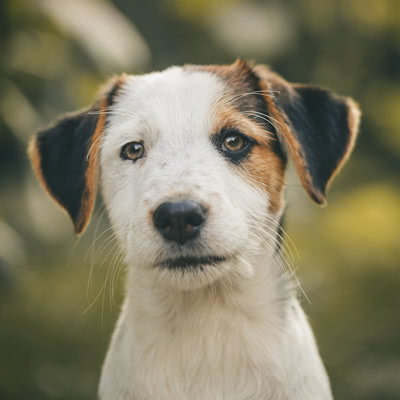
\includegraphics[width=0.5\textwidth]{figures/front_page/dog.jpg}\\
    %     \includegraphics[width=0.5\textwidth]{figures/front_page/molly.jpeg}\\
    %     \end{figure}
    %     \thispagestyle{empty}
    % \end{titlepage}

    \newpage
    \label{sec:eyyy}


    \section{Introduction}\label{sec:introduction}

Cell membranes are the foundation of the origin of life, but also linked to the dynamics of virus al infections and genetic mutations since it controls what substances that can exit or enter the cell \cite{ hurley2010membrane}. In fact, a good
understanding of the cell membrane is important of engineering proteins to manipulate various intracellular processes in living systems \cite{rojas1998genetic}.

One of the primary components of the cell membranes are lipids which serve many different functions. A key function is that it is consisting of a bilayer of lipids which controls the structural rigidity and the fluidity of the membrane. Thus, elastic
bending forces, temperature and diffusion is essential on how a cell membrane will evolve \cite{udo97,neidleman87}.


\subsection{Elastic bending energy on evolving surfaces}%
\label{sub:willmore_flow}

Assuming that the system is a single-phase system, i.e., the lipids are uniformly distributed, can the elastic bending energy be modelled using the Canham-Helrich energy functional \cite{helfrich1973elastic, wang08, udo97}. Let us denote $b_{b},
b_{k}$ and $H_{0}$ as parameters based on physical models, then can the energy functional be denoted as,
\begin{equation}
\label{eq:CH}
\mathcal{E} _{CH}\left( \Gamma\left( t \right)   \right) =   \int_{\Gamma  }^{}  b_{b} \left( H- H_{0} \right) ^{2} + b_{k} K
.\end{equation}
Here is $H =  \kappa_1 + \kappa_2 $ denoted as the mean curvature and $K = \kappa_1 \kappa_2$ as the gaussian curvature with respectively and $\kappa_1$ and $\kappa_2$ as principal curvatures. $\Gamma \left( t
\right) = \Gamma  $ is here an evolving surface in $\mathbb{R} ^3$, for more info see section \ref{sec:background}.  Using the Gauss-Bonnet theorem can it be shown that the problem above is equivalent to the so-called Willmore energy
functional \cite{montiel2009curves, willmore1996riemannian},

\begin{equation}
\label{eq:WE}
\mathcal{E} _{W} \left( \Gamma\left( t \right)   \right) = \int_{\Gamma  }^{} \frac{1}{2} H ^2
.\end{equation}

This is a well known problem in the mathematical community \cite{ topping2000towards, marques2014willmore,link2013gradient,kuwert2012willmore}. In fact, it is a mathematical tool used to study the geometry of surfaces because it can be used to study
the diffeomorphism from a initial surface to a minimal energy configuration, which are surfaces with the least possible area for a given boundary. This is important in many areas of mathematics, including differential geometry, topology and mathematical physics \cite{koerber2021area,jakob2022singularities, rupp21}.

It has been established many numerical methods for for shape optimization problems \cite{sokolowski1992introduction,ito2008variational}, evolving surface partial differential equations (PDE) \cite{dziuk2013finite, dziuk2007finite,
binz2022convergent, barrett2007parametric, barrett2007variational, kovacs2019convergent, lehrenfeld2018stabilized} and specific
algorithms for the Willmore energy problem \eqref{eq:WE} \cite{palmurella2022parametric, dziuk2008computational, bonito2010parametric,  kovacs2021convergent, hu2022evolving}.

\subsection{Two-phase separation modelling on predefined evolving surfaces }%
\label{sub:two_phase_seperation_modelling_on_surfaces_}

It also turns out that the lipids often accumulate into so-called lipid rafts which serves as a rigid platform for proteins with special properties such as intracellular trafficking of lipids and lipid-anchored proteins \cite{ miller2020divide}. Modelling of
lipid rafts formation can be modelled as a two-phase separation problem based on minimization of the Ginzburg-Landau energy functional \cite{yushutin19},
\begin{equation}
\label{eq:GL}
\mathcal{E}_{GL}  \left( c   \right) = \int_{\Gamma\left(t  \right)   }^{}\Psi \left( c \right) + \frac{\gamma}{2} \left\lvert \nabla c \right\rvert^{2} ,
\end{equation}
which describes the chemical energy for a concentration $c: \Gamma\left( t \right)  \times \left[ 0,T \right] \mapsto  \left[ 0,1 \right]  $. Here is $ \Psi \left( c \right): \mathbb{R} \mapsto \mathbb{R} $ denoted as a nonlinear scalar chemical potential function. Keep in mind that unlike
the Willmore energy functional \eqref{eq:WE}, where the $\Gamma\left( t \right)  $ is determined by the elastic properties, should the energy functional \eqref{eq:GL} be interpreted as a chemical diffusion problem a predefined evolving domain $\Gamma \left( t \right) $.
Usually is this problem solved by deriving equivalent variants of partial differential equations (PDE) such as Allen-Cahn equation (or Cahn-Hilliard equation if the total concentration is globally conserved) on evolving domains. For further details,
see \cite{yushutin19,
udo97, ratz16,Gera2017, caetano21, elliott2015evolving}.

\subsection{Multiphysics problems on evolving surfaces}%

Ultimately will the cell membrane consists of interaction several kinds of physics (temperature, elasticity, chemical diffusion, internal fluid pressure etc.) \cite{udo97}. Hence, being able to model several processes may give unforeseen results.

An interesting example is to couple the energy functionals \eqref{eq:GL}  and \eqref{eq:CH}, since the lipid-rafts formation is said to change the elasticity properties of the membrane, may be a good model for how cell membranes evolve to specific shapes or execute cell division. One way
to couple the energy functionals is to let the parameters $b_{b}, b_{k}$ and $ H_{0} $ be some function of the time dependent concentration $c$, i.e.,
\[
    \begin{split}
        \mathcal{E}_{CHGL} \left( \Gamma\left( t \right) ,c\left( t \right)    \right) =  & \int_{\Gamma  }^{}  b_{b}\left( c \right)  \left( H- H_{0}\left( c \right)  \right) ^{2}  \\
        & + \int_{\Gamma   }^{} b_{k}\left( c \right)  K \\
        &+ \int_{\Gamma   }^{}\Psi \left( c \right) + \frac{\gamma}{2} \left\lvert \nabla c \right\rvert^{2} ,
    \end{split}
\]
For more information, see \cite{elliott2010surface}.

Recently have some authors also coupled diffusion processes and the so-called mean curvature energy, see \cite{burger2021interaction, elliott2022numerical}. It is well known that lipids travels
along the cell membrane in a fluidic manner, hence, it is also of interest to couple the Ginzburg-Landau energy functional \eqref{eq:GL} (or more specifically the Cahn-Hilliard equation) with the Navier-Stokes equation. Some methods has been proposed
methods for solving the problem on surfaces
and evolving surfaces, but it remains a field of active research \cite{olshanskii2022comparison}. As far as a author knows, coupling the Canham-Helrich energy functional \eqref{eq:CH}, Ginzburg-Landau energy functional \eqref{eq:GL}  and Navier-Stokes equation remains a open problem.

Some physical processes may require constant area and volume. This can simply be added by introducing respectively area and volume functionals, see \cite[Definition 2.5]{muller2013volume}.

Until now have all the models assumed that the membrane has no difference in internal and external pressure. As a matter of fact, osmotic pressure can be introduced by adding a energy functional using the van't Hoff formula. Let $V_{p}$ be the volume
of a closed evolving surface $\Gamma \left( t \right) $, we can then model the difference of internal and external pressure as,
\[
\Delta P \left( V_{p} \right) = P_{in} - P_{out} = iRT\left( \frac{n}{V_{p}} - \overline{c}  \right),
\]
where $i, R, T, \overline{c} $ and $n$ are the van't Hoff index, ideal gass constant, temperature , ambient molar concentration and molar amount of the enclosed solute. Then the energy
functional have the form,
\[
\mathcal{E} _{p}\left( \Gamma    \right)  = \int_{\Gamma   }^{   } \Delta P\left( V_{p} \right) ,
\]
For more information, see \cite{zhu2022mem3dg}.


\subsection{Outline of this report}%
\label{sub:outline_of_this_report}

The long-term goal would be to solve the multi-physics problems above. However, many of the problems above is fairly complicated to solve numerically and requires sophisticated techniques. Hence, in this report we focus on the latest research withing
the numerical methods of finding the minima of the energy functional \eqref{eq:WE}. However, we will first establish notation by including a section for definitions and important results from differential geometry and shape derivatives. We will then derive the
underlying dynamics system of evolutionary system dynamics using the gradient flow technique inspired by shape optimization methods based on the work done in \cite{ dougan2012first}. Lastly, we will establish the numerical methods of the system
dynamics by applying recent methods using an evolutionary surface finite element method (FEM) \cite{kovacs2021convergent, hu2022evolving}.



    
\newpage
\section{Unfitted cut discontinuous Galerkin method for the Poisson equation}%
\label{sec:elliptic}

\subsection{Introduction}%
\label{sub:introduction}


\subsection{Notation}%
\label{sub:notation}

\subsection{Hilbert Spaces}%

\label{ssub:hilbert_spaces}
\begin{tcolorbox}
    This subsection is copied from the project thesis
\end{tcolorbox}

We will in this report assume $\Omega $ to be a compact and open set in $\mathbb{R} ^{2}$. Now let the parameter $p \in \mathbb{R} $, $p\ge 1$. We then define the space $L^{p}\left( \Omega  \right) $ to be the set of all measurable functions $f: \Omega  \mapsto \mathbb{R} $ such that
$\left\lvert f \right\rvert ^{p}$ is Lebesgue measurable, i.e,

\begin{equation*}
    L^{p}\left( \Omega  \right) = \left\{ f: \Omega \mapsto \mathbb{R}  \mid \int_{\Omega }^{} \left\lvert f \right\rvert ^{p} d \Omega  < \infty  \right\}
.\end{equation*}

A useful extension, which we will use later, are the set of locally integrable functions for any compact subset $K \subseteq \text{Interior}\left( \Omega  \right) $ \cite{brenner07math}, that is,

\begin{equation*}
    L_{loc}^{1}\left( \Omega  \right)  = \left\{ f: f \in L^{1}\left( \Omega  \right)  \quad \forall K  \right\}.
\end{equation*}
Let $u \in L^{p}\left( \Omega  \right) $. We define the integral norm of order $p$ to be \[
\| u \|_{ L^{p}\left( \Omega  \right)  }^{  }  = \left( \int_{\Omega }^{} \left\lvert u \right\rvert ^{p} dx  \right) ^{\frac{1}{p}}.
\]
Since $p=2$ is frequently used in this report, we also define for convenience a compact notation $\| u \|_{ \Omega  }^{  }  = \| u \|_{ L^{2}\left( \Omega  \right)  }^{  } $ .  We say that $L^{2}\left( \Omega  \right) $ is a Hilbert space if it is equipped with a inner
product of two functions $u,v \in L^{2}\left( \Omega  \right) $ such that
\[
\left( u,v \right) _{\Omega } = \left( u,v \right) _{L^2\left( \Omega  \right) } = \int_{\Omega }^{} u  v dx.
\]

To generalize, we denote the notation $\mathcal{V} $ for a arbitrary Hilbert space. Furthermore, we define the dual space the be the space of linear and bounded functionals $F: \mathcal{V}  \mapsto \mathbb{R} $\cite{quartdiff}, i.e., \[
\mathcal{V} ^{*} =
\left.
\begin{cases}
F: \mathcal{V}  \mapsto \mathbb{R} \text{ such that }\forall v,w \in \mathcal{V}, \forall a,b \in \mathbb{R} \text{ and } C> 0 \text{ is }   \\
  F\left( \lambda v + \mu w  \right) = \lambda F(v) + \mu F(w) \text{ and } \left\lvert F\left( v \right)  \right\rvert \le C \| v \|_{ \mathcal{V}  }^{  }
\end{cases}
  \right\}
\]
and we equip it with the functional norm,  \[
    \| F \|_{ \mathcal{V} ^{*} }^{  } = \sup_{v \in \mathcal{V}   } \frac{\left\lvert F\left( v \right)  \right\rvert }{\| v \|_{ \mathcal{V}  }^{  } }.
\]

We will now establish a notion of the weak derivative, but first are we going to characterize some useful definitions of continuity. The space $C^{k}\left( \Omega  \right) $ for $k\ge 0$ denotes the set of functions whose derivatives, up to order of
$k$ , is continuous in $\Omega $. Note that we often use the shorthand notation $ C^{0} = C\left( \Omega  \right)  = C^{0}\left( \Omega  \right) $.
From this, let $C^{\infty}\left( \Omega  \right) $ be the set of infinitely differentiable functions in $\Omega $. Furthermore, we then denote the space $C^{\infty}_{0}\left( \Omega  \right)$ as the space of all functions, $u \in C^{\infty}\left( \Omega
\right) $, vanishing outside of any compact subset of $\Omega $. Let $u,v \in  C^{1}\left( \Omega  \right) $ and the define boundary $\Gamma  = \partial \Omega $ with a corresponding outer normal vector $n$. It is well known that this partial
integration formula holds \cite{manzoni2021optimal},

\[
\int_{\Omega }^{} \nabla u \cdot v dx = \int_{\Gamma }^{} u\cdot v n ds - \int_{\Omega }^{} u \cdot \nabla v dx.
\]
We now use this notation for derivatives
\footnote{In literature is often $D^{\alpha } f$ commonly used, but later in the report is this notation reserved for the Hessian operator. Therefore, we then the notation $\partial ^{\alpha } f$ in this report.} so
\begin{equation}
\label{eq:mixed_derivative}
\partial ^{\alpha  } f = \frac{\partial ^{\left\lvert \alpha  \right\rvert } f}{ \partial ^{\alpha _{1} } x_{1} \partial ^{\alpha _{2}} x_{2}  }, \quad \text{where } \alpha=\left( \alpha _{1}, \alpha _{2} \right) \text{ and } f \in C^{\left\lvert \alpha  \right\rvert }
\left( \Omega  \right)
.\end{equation}
Finally, let $u \in  L^{1}_{loc}\left( \Omega  \right) $. We call the function $w \in L_{loc}^{1}\left( \Omega  \right) $ the $\alpha $-th weak derivative of $u$  if \[
\int_{\Omega }^{} w \varphi  dx = \left( -1 \right) ^{\left\lvert \alpha  \right\rvert } \int_{\Omega }^{} u \cdot \partial ^{\alpha } \varphi dx, \quad \forall \varphi \in  C_{0}^{\infty}\left( \Omega  \right).
\]

We are now able to construct the Sobolev space \cite{manzoni2021optimal}, \[
H^{m}\left( \Omega  \right) = \left\{ u \in L^{2}\left( \Omega  \right)  \mid  \partial ^{\alpha } u \in L^{2}\left( \Omega  \right)  \forall \alpha : \left\lvert \alpha  \right\rvert  \le m \right\} \text{ for } m>1
\]
Equipped with the inner product is $H^{m}\left( \Omega  \right) $  denoted as a Hilbert space, that is, for $u,v \in H^{m}\left( \Omega  \right) $, \[
    \left( u,v \right) _{H^{m}\left( \Omega   \right) } = \sum_{\left\lvert \alpha  \right\rvert  \le  m}^{}  \int_{\Omega }^{} \partial ^{\alpha } u \partial ^{\alpha } v dx.
\]
Similarly, the integral norm is denoted as, \[
\| u \|_{ H^{m}\left( \Omega  \right)  }^{  }  = \left( \| u \|_{ L^{2}\left( \Omega  \right)    } + \sum_{k = 1}^{m}  \left\lvert u \right\rvert ^{2} _{  H^{k}\left( \Omega  \right) }\right) ^{\frac{1}{2}},
\]
where the seminorm is defined such that, \[
\left\lvert u \right\rvert _{H^{k}\left( \Omega  \right) } = \left( \sum_{\left\lvert \alpha  \right\rvert  = k}^{} \| \partial ^{\alpha }u \|_{ \Omega  }^{ 2 }  \right).
\]
For convenience, we also entitle the notation,
\[
H^{m}_{0} \left( \Omega  \right) = \left\{ \text{completion of }C_{0}^{\infty}\left( \Omega  \right) \text{ w.r.t. } \| \cdot  \|_{H^{m}\left( \Omega  \right)   }^{  }  \right\}.
\]
\todo[inline]{ Write definitions considering $H^{\frac{1}{2}}( \Gamma ) $  }


\subsection{Possion problem}%
\label{sub:possion_problem}

Let $f \in H^1( \Omega ) $ and $g \in H^{\frac{1}{2}}( \Gamma ) $ and $\Omega  \in \mathbb{R} ^{d}$ . We then define the strong formulation of the Possion problem to be \[
\begin{split}
    -\Delta u &= f \in \Omega  \\
     u &= g \in \Omega  \\
\end{split} .
\]
Let us define the Hilbert spaces $V=H^{1}( \Omega ) $,   $V_{g} = \left\{ v \in H^{1}( \Omega ): v \mid _{\Gamma } = g \right\} $, the bilinear form $a: V \times V  \to \mathbb{R}  $ and the linear form $l: V'\to \mathbb{R}  $ s.t. \[
a( u,v) = ( \nabla u, \nabla v) _{\Omega }, \quad l( v) = (f,v)_{\Omega }.
\]
We say the weak formulation is to find a $u \in V_{g}$ so this equation holds  \[
a( u,v) = l( v), \quad  \forall v \in V
\]









    % 
\newpage
\section{Biharmonic equation}%
\label{sec:cahn_hilliard_equation}


Let $c_0$ and $c_1$  indicate the concentration profile of the substances in a $2$ -phase system such
that $c_0 \left( \mathbf{x},t \right): \Omega  \times \left[ 0, \infty \right] \to \left[ 0,1 \right]$ and
similarly $c_1 \left( \mathbf{x},t \right): \Omega \times \left[ 0, \infty \right] \to \left[ 0,1 \right]$, where
$\mathbf{x} $ is a element of some surface $\Omega $ and $t$ is time.
However, in the $2$ phase problem will we will restrict ourself so that $c_0\left( t,\mathbf{x} \right) + c_1\left( t,
\mathbf{x} \right) = 1$ at any $\mathbf{x} $ at time $t$. A property of the restriction is that we now can express
$c_0$ using $c_1$, with no loss of information. Hence, let us now define $c = c_0$ so $c \left( \mathbf{x},t \right):
\Omega  \times \left[ 0, \infty \right] \to \left[ 0,1 \right]$. It has been shown that $2$ phase system if
thermodynamically unstable can be evolve
into a phase separation
described by a evolutional differential equation \cite{cahnhilliard1957} using a model based on chemical energy of the
substances. However, further development has been done \cite{yushutin19} to solve this equation on surfaces. Now assume
model that we want to describe is a phase-separation on a closed membrane surface $\Gamma $, so that $c \left( \mathbf{x},t \right):
\Gamma \times \left[ 0, T \right] \to \left[ 0,1 \right]$. Then is the surface Cahn Hilliard equation described such that

\begin{equation}
    \label{eq:cahn1}
\rho \frac{\partial c}{\partial  t}  - \nabla_{\Gamma } \left( M \nabla _{\Gamma } \left( f_{0}'  - \varepsilon ^2
        \nabla^2
_{\Gamma } c \right) \right) = 0  \quad \text{on } \Gamma
.\end{equation}
We define here the tangential gradient operator to be $\nabla _{\Gamma } c = \nabla c - \left( \mathbf{n} \nabla c
\right)\mathbf{n} $ applied on the surface $\Gamma $ restricted to $\mathbf{n} \cdot \nabla _{\Gamma } c = 0$.

Lets define $\varepsilon $ to be the size of the layer between the substances $c_{1}$ and $c_{2}$. The density $\rho $ is
simply defined such that $\rho = \frac{m}{S_{\Gamma }}$ is a constant based on the total mass divided by the total
surface area of $\Gamma $.
Here is the mobility $M$ often derived such that is is dependent on $c$ and is crucial for the result during a possible
coarsening event \cite{yushutin19}.  However, the free energy per unit surface
$f_{0} = f_{0}\left( c \right)$ is derived based on the thermodynamical model and should according to \cite{yushutin19} be non convex and
nonlinear.

A important observation is that equation \eqref{eq:cahn1} is a fourth order equation which makes it more challenging to
solve using conventional FEM methods. This clear when writing the equation on the equivalent weak form and second order
equations arise.


\newpage
\section{Energy Functionals}%
\label{sec:energy_functionals}
Let $c\left( x,t \right)  : \Gamma \times [0,T] \mapsto [0,1] $. From \cite{yushutin19} can we observe the energy functionals
\begin{equation*}
   E _{1}(c) = \int_\Gamma f(c)
.\end{equation*}
where \[
f\left( c \right) = f_{0}\left( c \right) + \frac{1}{2}\varepsilon ^{2} \left\lvert \nabla _{\Gamma } c \right\rvert ^{2}
\]
and the conservation law  $\rho \frac{\partial c}{\partial  t}  + div_{\Gamma } \mathbf{j} = 0$ for the evolution of  $c $, derived from the Ficks Law $\mathbf{j} = - M \nabla _{\Gamma } \mu $ for the chemical potential derived by the functional derivative $\mu = \frac{\delta
f}{\delta c} $. The double well function is denoted as \[
f_{0}\left( c \right)  = \frac{\zeta}{4} c^2(1- c)^2
\]






\newpage


    % 
\newpage
\section{Linear Cahn-Hilliard equation}%
\label{sec:linear_cahn_hilliard_equation}



\newpage


    % 
\newpage
\section{Applications to the Cahn Hilliard equation }%
\label{sec:cahn_hilliar_applications}

In this section, we will demonstrate that the proposed cut finite element method can be used to solve the Cahn-Hilliard problem. Firstly, we will recall the strong form and illustrate how it can be recast into a weak form following the approach in
\cite{feng2007fully}. Subsequently, we will derive a simplistic numerical time iteration scheme to demonstrate that the solution to the problem can indeed be found. Again, all numerical experiments are conducted using the open-source finite element method (FEM) framework, Gridap, as documented in \cite{verdugo22}.


\subsection{Deriving the discrete formulation of the Cahn-Hilliard equation}%
\label{sub:revisiting_the_strong_formulation}

 Recall the strong formulation of the Cahn-Hilliard equation.
Let $ u( x,0) =  u_{0}$ then is the dynamics on the form,
\begin{subequations}
\label{eq:strong_ch}
    \begin{align}
\partial _{t} u + \Delta  \left(  \varepsilon^2  \Delta u - f( u) \right)   &=0  \quad \text{ in } \Omega  \\
\partial _{n} u &= 0 \quad \text{ on } \Gamma  \\
\partial _{n}    \Delta u       &= 0 \quad \text{ on } \Gamma
    \end{align}
\end{subequations}
Here we define $f( u) = u( u^{2} -1)  = F' ( u)  $ where $F( u) = ( 1 / 4 ) ( u^2 -1 ) ^{2} $. With the corresponding energy. We define the small parameter to be $\varepsilon  = 1 / 100$.
\begin{equation}
    \label{eq:physical_prop}
E( u)  = \int_{\Omega }^{} \frac{\varepsilon^{2} }{2} \abs{ \nabla u } ^2 +  F( u) dx
\end{equation}

We also recall that the energy functional monotonically decreasing and that the global mass concentration is conserved, i.e.
\begin{equation}
\label{eq:mass_cons_energy_decrease2}
\frac{d}{dt} E( u)  <  0 \text{ and }\frac{d}{dt} \int_{\Omega }^{}  u dx = 0.
\end{equation}

For convenience, we decompose the functional so that $E(u) = E_{1}(u) + E_{2}(u)$. Here, $E_{1}(u) = \int_{\Omega } \frac{\varepsilon^{2}}{2} |\nabla u|^2 , dx$ represents the smoothing contribution, while $E_{2}(u) = \int_{\Omega } F(u) , dx$ represents the separation contribution.

Now assume that $u \in L^2( [0,T], H^{4}( \Omega ) ) $ and $v_{h} \in  V_{h}$ of order $k$. It is clear that the initial weak formulation is,
\begin{equation}
    ( \partial_{t} u,v_{h} )_{\Omega }  + \varepsilon^{2} ( \Delta ^2u, v_{h})_{\Omega } -  ( f( u), v_{h} )_{\Omega } = 0.
\end{equation}

As we can see did the biharmonic equation appear and, thus, we can apply the cut finite element framework developed in Section \ref{sec:cutcip_biharmonic_problem}. We define the discrete weak problem as follows.
\begin{equation}
    \begin{split}
        & \text{Find  }u_{h} \in L^{2}( [0,T],V_{h})  \text{ such that } \forall v_{h} \in V_{h} \\
        & ( \partial_{t} u_{h},v_{h} )_{\Omega }   + \varepsilon^{2} A_{h}( u_{h},v_{h})   +  c_{h}( u_{h},v_{h})  = 0.
    \end{split}
\end{equation}
Here we have followed the nonlinear weak formulation \cite[Equation
4.2]{feng2007fully} and the cut finite element bilinear form for the biharmonic equation proposed in Equation \eqref{eq:discrete_CutCIP_prob} such that
\begin{align}
    c_{h}( u_{h}, v_{h})  & = ( f( u_{h}) ,\Delta v_{h})_{\Omega } +  ( f( u_{h}) , \partial _{n}v)_{\mathcal{F}_{h} } \\
    A_{h}( u_{h}, v_{h})  & =  a_{h}( u_{h}, v_{h}) + g_{h}( u_{h}, v_{h})
\end{align}

The primary aim is to formulate demonstrate that this problem can be solved using a simple time-integration scheme. Define the index $m= 0, 1, \ldots, M$. This index corresponds to uniformly distributed time points $t_{m}$, which are subject to the
boundary conditions $t_{0} = 0$ and $t_{M} = M \tau$. Here, we denote the time step as $\tau = \varepsilon^2$. Each time step $u^{m}_{h}$ is an element of the discrete space $V_{h}$ , i.e. $u^{m}_{h} \in V_{h}$  with the initial condition defined as $u^{0} = u( t_{0},x )$. Following this, we establish the forward difference operator, which is determined by the time step $\tau $.
\begin{equation}
\overline{\partial } _{t} u_{h}^{m} = \frac{u_{h}^{m} - u_{h}^{m-1}}{ \tau }
\end{equation}

We define the Implicit explicit scheme (IMEX) scheme to have the following discretization,
\begin{equation}
( \overline{\partial } _{t} u^{m}_{h}, v_{h}   )_{\Omega } + \varepsilon^{2} A^{m}_{h}( u_{h}^{m} , v) +  c_{h} (  u_{h}^{m-1}, v_{h})  = 0 , \quad \forall v_{h}, u^{m}_{h} \in V^{}_{h}.
\end{equation}
which equivalently can be rewritten as
\begin{equation}
( u_{h}^{m},v )_{\Omega }  + \tau \varepsilon^{2} A_{h}( u_{h}^{m} , v)   =  ( u_{h}^{m-1},v )_{\Omega } - \tau c_{h} (  u_{h}^{m-1}, v) .
\end{equation}
Hence, we have a complete space time scheme.


\subsection{Demonstration on the Cahn-Hilliard problem}%
\label{sub:demonstration_on_the_physical_cahn_hilliard}

For the strong form of the Cahn-Hilliard \eqref{eq:strong_ch} we have no analytical solution, so we cannot construct a manufactured solution. However, a way to check that the system does behave like expected based on the physical properties \eqref{eq:physical_prop}. In other
words, we can check that our discrete solution satisfies the following conditions. We define the discrete values $E^m = E( u_{h}^{m})$, $E_{1}^m = E_{1}( u_{h}^{m})$ and $E_{2}^m = E_{2}( u_{h}^{m})$ and the initial function  $u_{0} = u( x,0) $. From
the physical properties \eqref{eq:physical_prop} to we expect the discrete equivalent to hold, i.e.
\begin{equation}
    E^m   <  E^{ m-1 } \text{ and }   \int_{\Omega }^{} u_{h}^{m}   dx \approx \int_{\Omega }^{} u_{0}  dx.
\end{equation}
To test this, we check that $ \delta E^{m} >0 $ generally holds, where
\begin{equation}
 \delta E^{m} = E( u_{h}^{m-1}) -  E( u_{h}^{m}) ,  \\
\end{equation}
 Similarly, let us define the relative cumulative global mass error and local mass error.
 \begin{equation}
 \Delta u_{h}^{m}  = \frac{ \abs{ \int_{\Omega }^{}  ( u_h^{m} - u_{0} ) dx } }{ \abs{ \int_{\Omega }^{}  u_{0} dx } } \quad \text{ and } \quad
 \delta u_{h}^{m}  = \frac{  \int_{\Omega }^{}  ( u_h^{m} - u^{m-1}_{h} ) dx  }{ \abs{ \int_{\Omega }^{}  u_{0} dx } }.
 \end{equation}
 To test mass conservation we expect the error $\Delta u_{h}^{m}$ and $\delta u_{h}^{m}$   to be close to zero.

\begin{figure}[]
    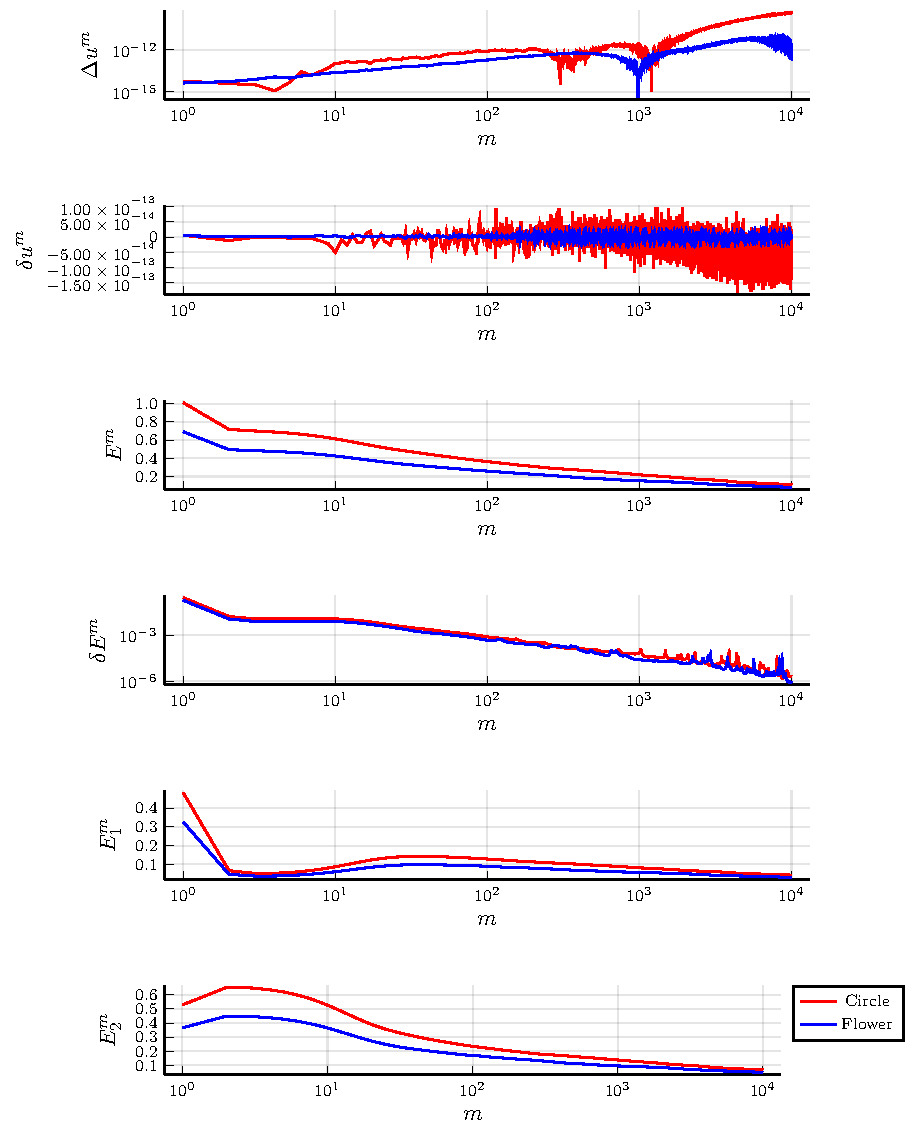
\includegraphics{results/physical_CH_plot.pdf}
    \caption{Evolution of the  global mass conservation $\Delta u^m$, and the local mass difference $\delta u^m$ total discrete energies $E^m$,$E^m_{1}$,$E^m_{2}$, with the corresponding local energy difference $\delta E^m$, on a circular domain and a flower-shaped domain. }
    \label{fig:physical_CH_plot}
\end{figure}


\begin{figure}[]
    \centering
    \hfill
    \subfloat[$m=0$]{
        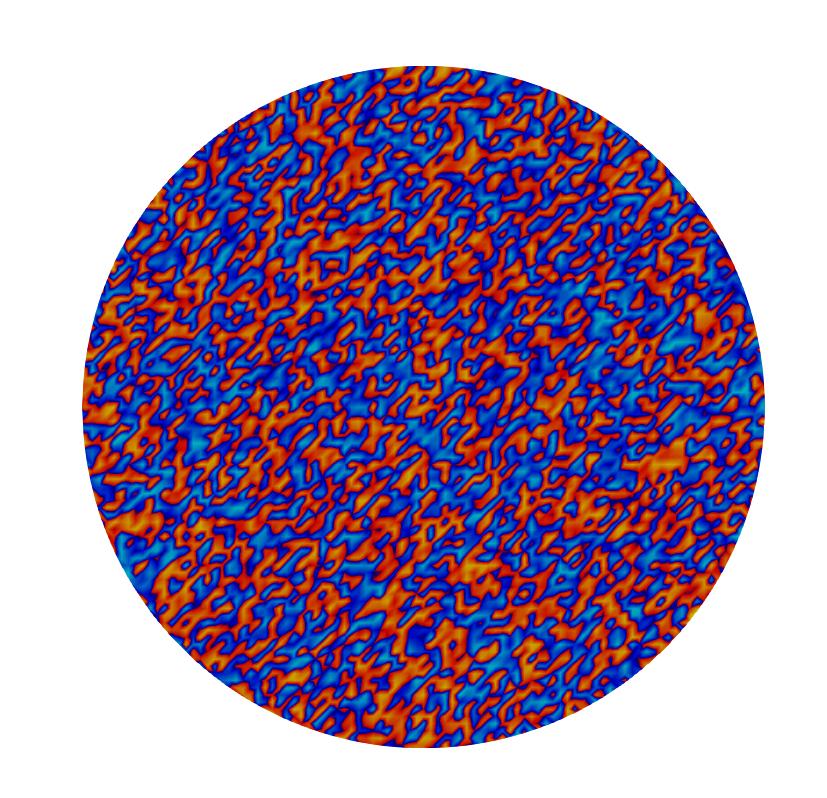
\includegraphics[width=0.3\textwidth]{results/illustration/c0.png}
    }\hfill
    \subfloat[$m=2$]{
        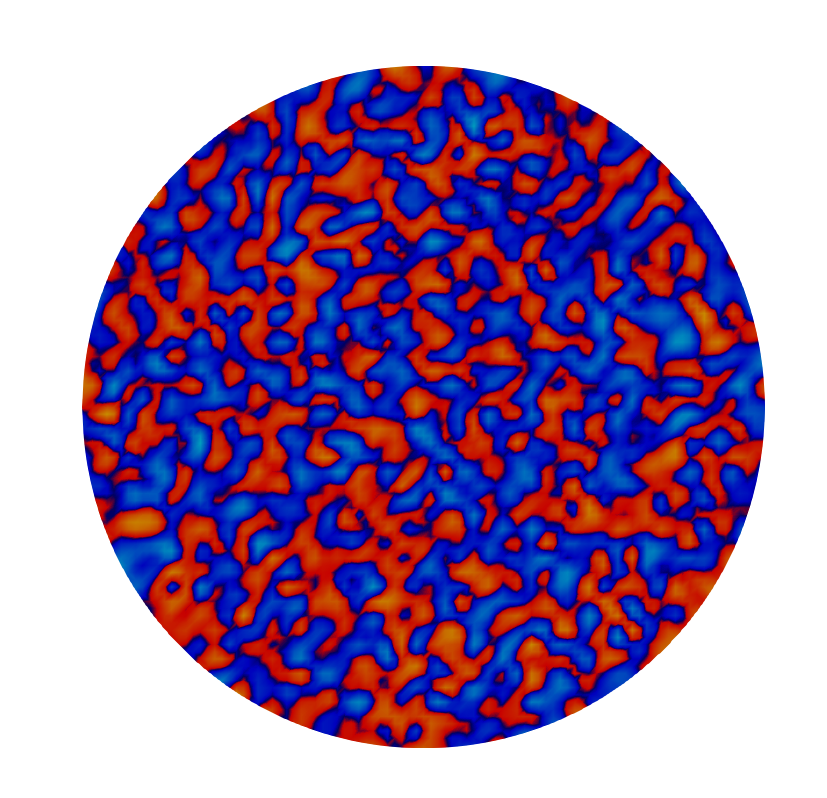
\includegraphics[width=0.3\textwidth]{results/illustration/c2.png}
    }
    \hfill
    \subfloat[$m=10$]{
        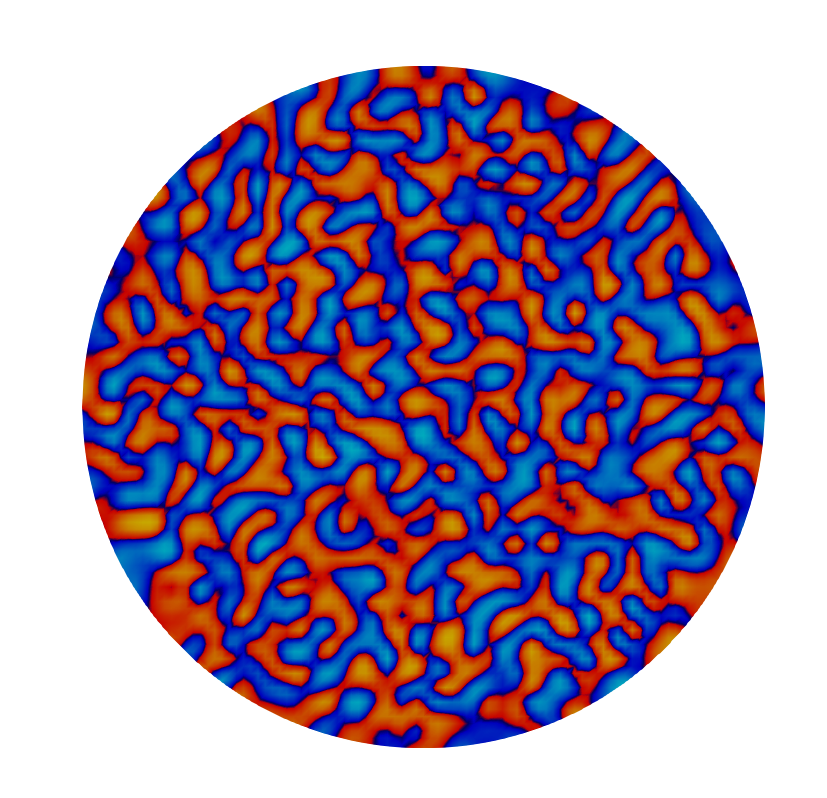
\includegraphics[width=0.3\textwidth]{results/illustration/c10.png}
    }
    \\
    \vspace{10pt}
    \hfill
    \subfloat[$m=50$]{
        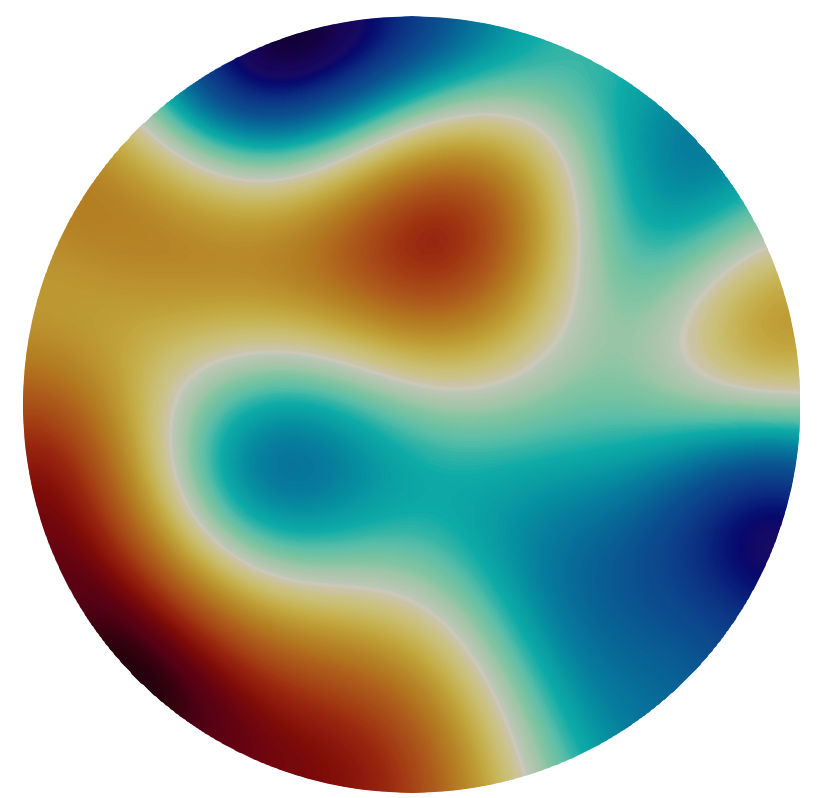
\includegraphics[width=0.3\textwidth]{results/illustration/c50.png}
    }
    \hfill
    \subfloat[$m=200$]{
        
\includegraphics[width=0.3\textwidth]{results/illustration/c200.png}
    }\hfill
    \subfloat[$m=500$]{
        
\includegraphics[width=0.3\textwidth]{results/illustration/c500.png}
    }
    \\
    \vspace{10pt}
    \hfill
    \subfloat[$m=1000$]{
        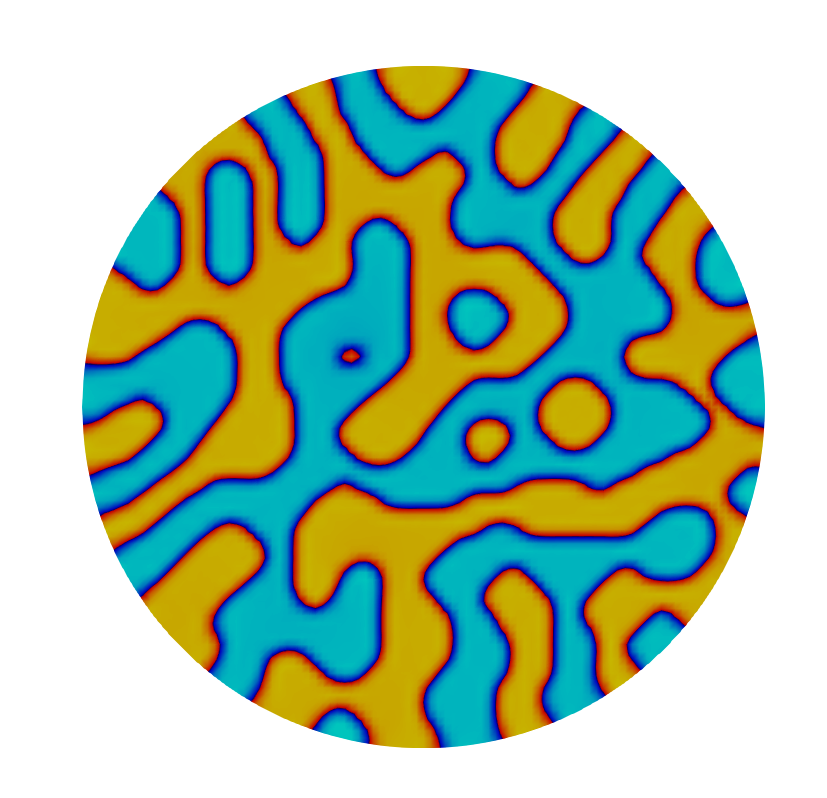
\includegraphics[width=0.3\textwidth]{results/illustration/c1000.png}
    }
    \hfill
    \subfloat[$m=5000$]{
        
\includegraphics[width=0.3\textwidth]{results/illustration/c5000.png}
    }\hfill
    \subfloat[$m=10000$]{
        
\includegraphics[width=0.3\textwidth]{results/illustration/c10000.png}
    }
    \vspace{10pt}
        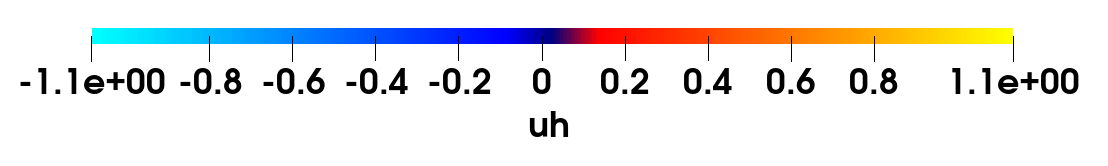
\includegraphics[width=0.8\textwidth]{results/illustration/colobar.png}

    \caption{Illustration of simulations of the Cahn-Hilliard equation on the circle domain for $t\in \left[ 0, 10000\tau  \right] $.}
        \label{sub:fig:ill_circle}
\end{figure}

\begin{figure}[]
    \centering
    \hfill
    \subfloat[$m=0$]{
        
\includegraphics[width=0.3\textwidth]{results/illustration/f0.png}
    }\hfill
    \subfloat[$m=2$]{
        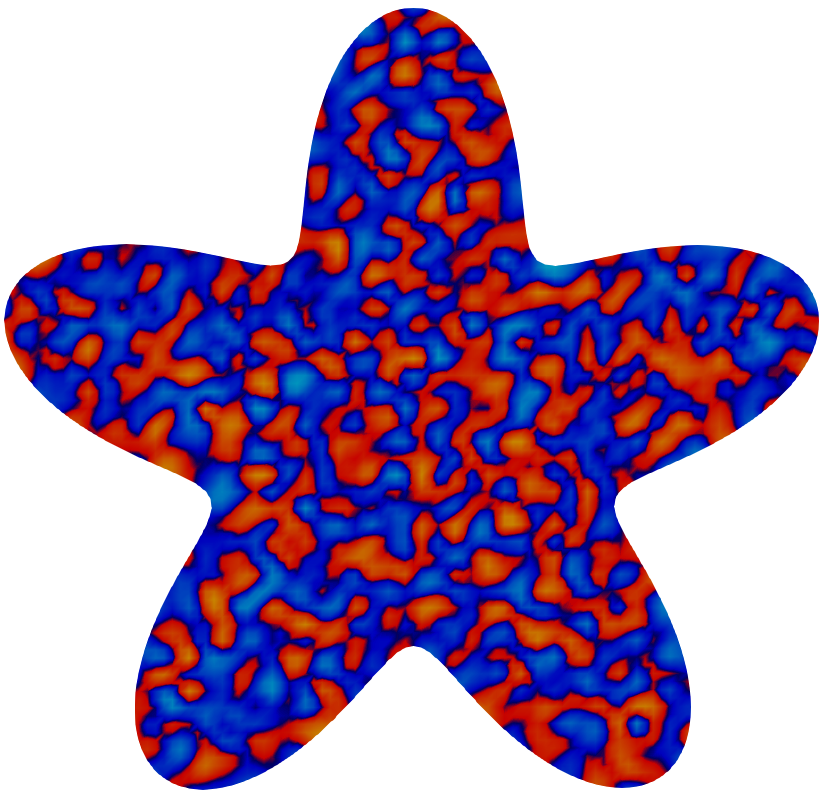
\includegraphics[width=0.3\textwidth]{results/illustration/f2.png}
    }
    \hfill
    \subfloat[$m=10$]{
        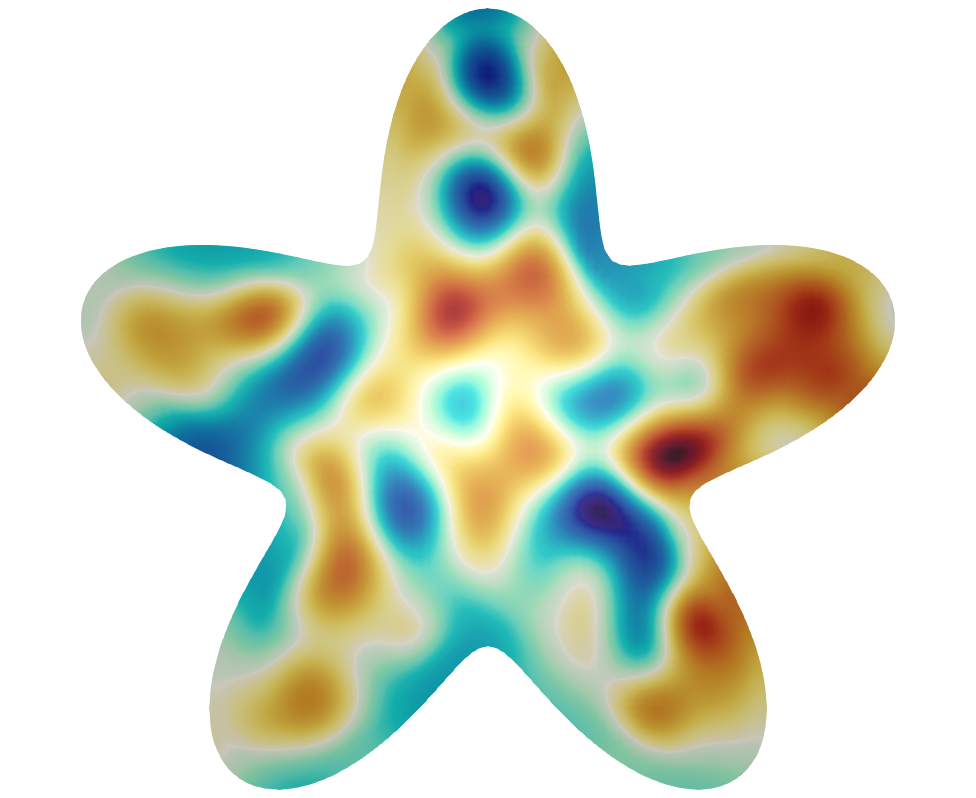
\includegraphics[width=0.3\textwidth]{results/illustration/f10.png}
    }
    \\
    \vspace{10pt}
    \hfill
    \subfloat[$m=50$]{
        
\includegraphics[width=0.3\textwidth]{results/illustration/f50.png}
    }
    \hfill
    \subfloat[$m=200$]{
        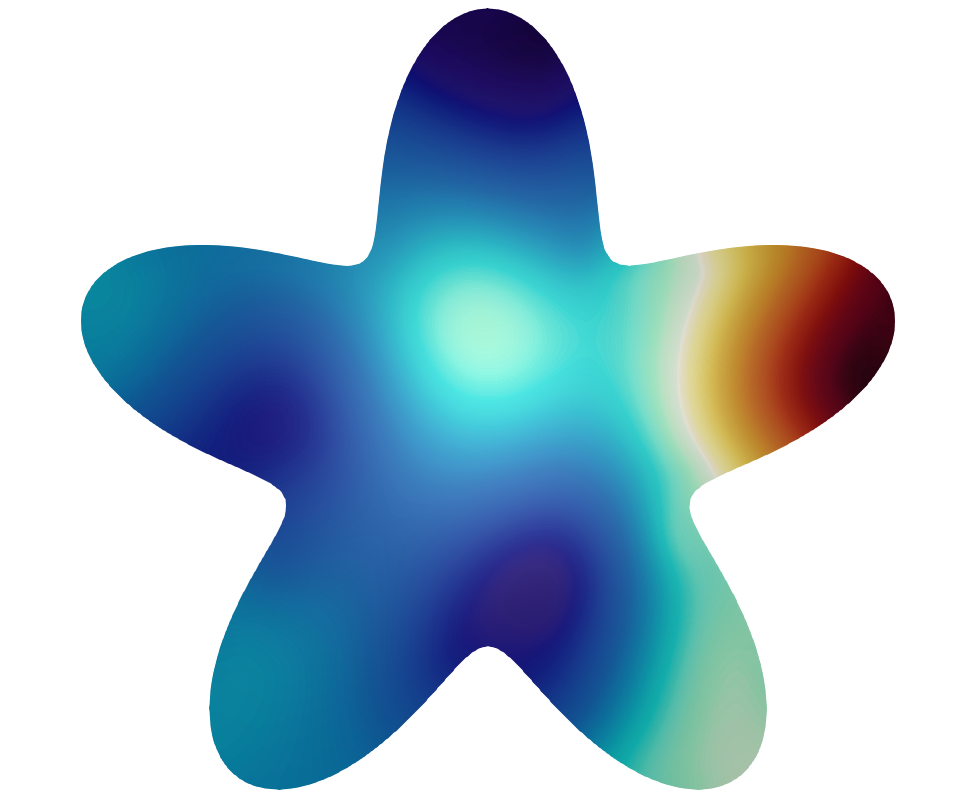
\includegraphics[width=0.3\textwidth]{results/illustration/f200.png}
    }\hfill
    \subfloat[$m=500$]{
        
\includegraphics[width=0.3\textwidth]{results/illustration/f500.png}
    }
    \\
    \vspace{10pt}
    \hfill
    \subfloat[$m=1000$]{
        
\includegraphics[width=0.3\textwidth]{results/illustration/f1000.png}
    }
    \hfill
    \subfloat[$m=5000$]{
        
\includegraphics[width=0.3\textwidth]{results/illustration/f5000.png}
    }\hfill
    \subfloat[$m=10000$]{
        
\includegraphics[width=0.3\textwidth]{results/illustration/f10000.png}
    }
    \vspace{10pt}
        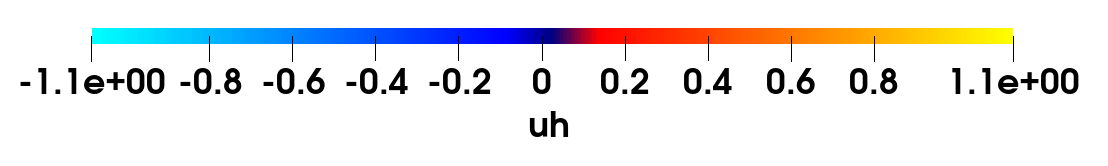
\includegraphics[width=0.8\textwidth]{results/illustration/colobar.png}
    \caption{Illustration of simulations of the Cahn-Hilliard equation on the flower domain for $t\in \left[ 0, 10000\tau  \right] $.}
        \label{sub:fig:ill_flower}
\end{figure}



In our experiments, we defined the initial function $u_{0}(x)$ as the uniform samples from the interval $[-1, 1]$ for each node. That is, for each node $a_{i}$, $u_{0}(a_{i})$ is a sample from the uniform distribution on the interval $[-1, 1]$. This
applies for all $i = 1, \ldots, N$, where $N$ is the total number of degrees of freedom in our system. The node $a_{i}$ is associated with the nodal basis for all $N$ degrees of freedom, as discussed for the discrete system
\eqref{eq:discretized_system}. We again used a square background mesh with length $L=2.7$ and mesh size $h=\frac{L}{n}$ for $n=2^{7}$. For an illustration of the active set $\mathcal{T}_{h} $ (defined in Section \ref{sub:unfitted_mesh}), see Figure \ref{sub:fig:active_mesh}.

\begin{figure}[H]
    \centering
    \hfill
    % \subfloat[]{
        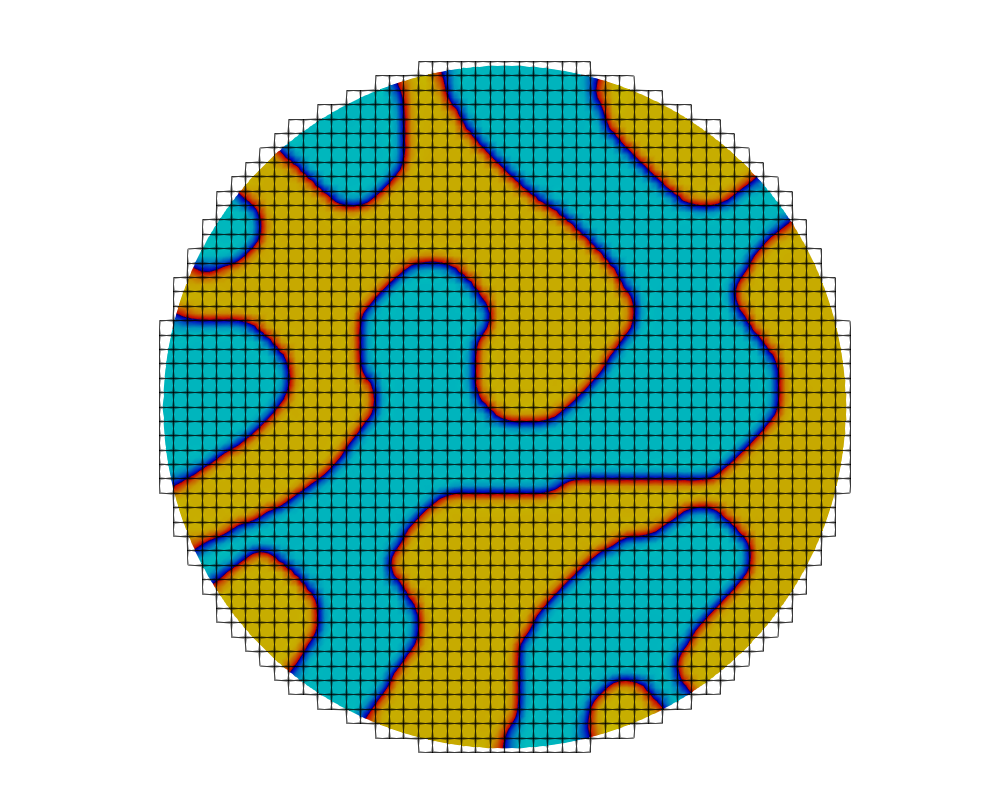
\includegraphics[width=0.45\textwidth]{results/illustration/active_circle.png}
    % }
    \hfill
    % \subfloat[]{
        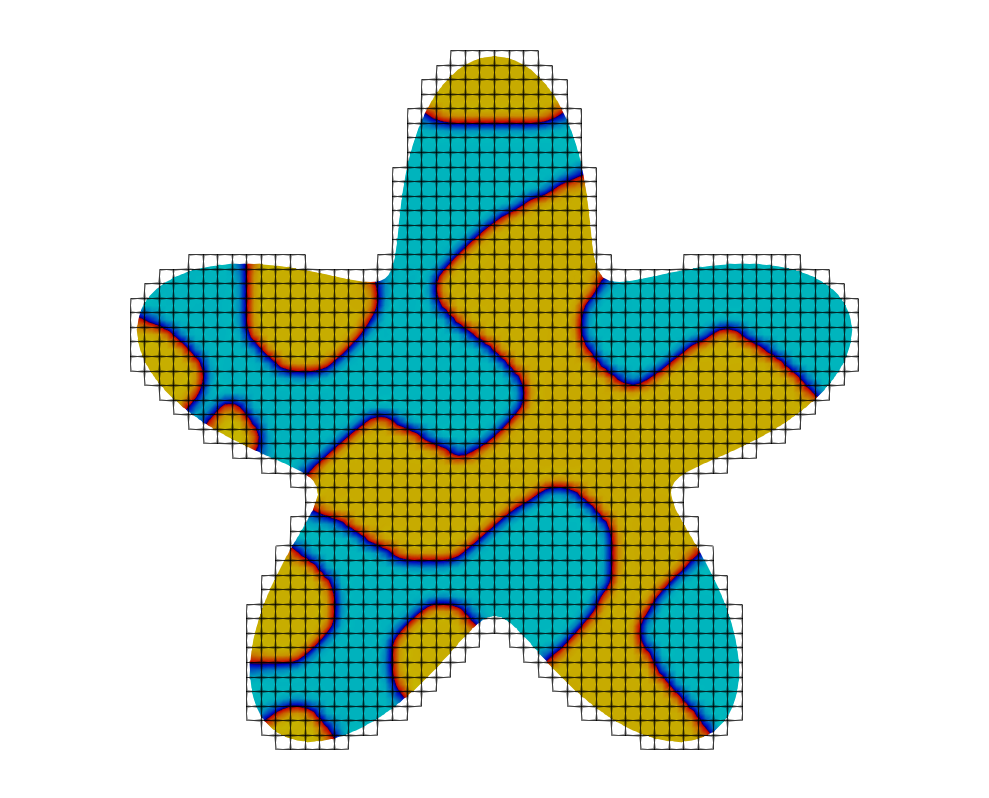
\includegraphics[width=0.45\textwidth]{results/illustration/active_flower.png}
    % }
    \caption{Illustration of the active mesh $\mathcal{T}_{h} $.}
    \label{sub:fig:active_mesh}
\end{figure}


We ran the simulation on the for the flower domain \eqref{eq:flower} and the circular domain \eqref{eq:circle}, illustrated in Figure \ref{sub:fig:ill_flower} and \ref{sub:fig:ill_circle}. The corresponding plots of the mass conservation and energy decrease are presented
in the Figure \ref{fig:physical_CH_plot}, and confirm the expected physical properties of the Cahn-Hilliard equation. The global relative error $\Delta u^{m}_{h}$ and $\delta u^{m}_{h}$ demonstrating that the mass is conserved. We also observe that the energy functional
$E(u_h)$ monotonically decreases over time and that $\delta E^{m} >0$, signifying the systems tendency to seek a state of minimal energy. Take note that $E^{m}{1}$ and $E^{m}{2}$ are interconnected in such a way that if the value of one increases, the other will correspondingly decrease to maintain balance, and vice versa.



\subsection{Note on the manufactured solution}%
\label{sub:the_problem}

While the report is not consisting of a numerical convergence analysis of the Cahn-Hilliard problem, we still present a framework for manufactured solutions for non-homogeneous boundary conditions. Let $ u( x,0) =  u_{0}$ then is Cahn-Hilliard with
non-homogeneous boundary conditions as follows,
\begin{subequations}
    \label{eq:ch_gen}
    \begin{align}
    \label{eq:ch_gen:a}
        \partial _{t} u + \Delta  \left(  \varepsilon^2  \Delta u - f( u) \right)   &= g_{0}( x)   \quad \text{ in } \Omega,  \\
        \partial _{n} u &= g_{1}( x)  \quad \text{ on } \Gamma,  \\
        \partial _{n}    \Delta u   &= g_{2}(x)  \quad \text{ on } \Gamma,
    \end{align}
\end{subequations}
where we defined $f( u) = F'( u) =u( u^2 -1)  $ for $F( u) = \frac{1}{4}( u^{2} - 1)^{2} $ and the domain $\Omega \subset \mathbb{R} ^{d} $  for $d = 2,3$. In contrast to the standard version presented in the introduction \eqref{eq:strongch}, this
version is generalized to also holds for for functions $g_{0},g_{1},g_{2}: \Omega \to\mathbb{R}   $. While the standard version may be physical correct, this version creates flexibility so we can easily construct manufactured solution on complex domains.

    Designing a manufactured solution using $g_{0}( \cdot ) $ may be temping with the formulation \eqref{eq:ch_gen:a}. However, observe that expanding the Laplacian we get,
    \begin{equation}
    \begin{split}
        \Delta  \left(  \varepsilon^2  \Delta u - f( u) \right) & = \varepsilon^2 \Delta^2 u -  \Delta f( u) \\
                                                                                    &= \varepsilon^{2} \Delta ^2 u  - 3( 2u \| \nabla u \|_{ 2 }^{ 2 } + u^{2}  \Delta u )   \\
    \end{split}
    \end{equation}
Here we applied the chain rule twice and inserted the derivatives.
\begin{equation}
    \label{eq:nonlinear_laplace}
    \begin{split}
\Delta f( u)  &= \nabla \cdot \nabla f( u)  = \nabla \cdot  \left[ f' ( u) \partial _{x_{1}}u, \ldots, f' ( u) \partial _{x_{d}}u \right] ^{T} \\
& =  f'' ( u)( ( \partial _{x_{1}}u )^{2} + \ldots +( \partial _{x_{d}}u )^{2} ) +  f' ( u)( \partial _{x_{1} x_{1}}u + \ldots +   \partial _{x_{d} x_{d}}u ) \\
&=  f'' ( u) \| \nabla u \|_{ 2 }^{ 2 } + f' ( u)  \Delta u  = 6u \| \nabla u \|_{ 2 }^{ 2 } + 3u^{2}  \Delta u
    \end{split}
\end{equation}

% Our goal is to write the Cahn Hilliard equation on weak form.
% Assume that $\Omega  \subset \mathbb{R} ^{d}$ with a $\Gamma $ in $C^2$.
%  Let $u \in  H^{4}( \Omega ) $ and $v \in V_{h} $.
% Now, expanding the first Laplace operator from a weak point of view is it clear that
% \[
%  ( \Delta ( \varepsilon  \Delta u - \frac{1}{\varepsilon } f( u) ) ,v )_{\Omega } = \varepsilon ( \Delta^{2} u ,v )_{\Omega } - \frac{1}{\varepsilon } ( \Delta f( u)  ,v )_{\Omega }.
% \]
% Hence, this makes it natural to associate the biharmonic $( \Delta ^2 u,v)_{\Omega } $ with bilinear forms $A_{h}( \cdot ,\cdot ) $ , however, in this section will we only consider the Laplace
% variant $a^{L}( \cdot ,\cdot ) $.
We now seek to find a weak form of the nonlinear term with non homogeneous boundary conditions.
\begin{lemma}[Semi-linear form]
    Let $u \in H^4( \Omega ) $ be solution to \eqref{eq:ch_gen} and $v_{h} \in V_{h}$ the test function.
Then can we rewrite the nonlinear term into the corresponding semi-linear form $c_{h}( \cdot ,\cdot )  $ for the nonlinear term $( -\Delta f( u) , v_{h})_{\Omega }$ into two consistent formulations.
\begin{align}
    \label{eq:ch:1}
      c^{1}_{h} ( u,v_{h})  & = ( f' ( u) \nabla u, \nabla v_{h} )_{\Omega }  - ( f'( u)  g_{1}   ,  v_{h})_{\Gamma } \\
    \label{eq:ch:2}
        c^{2}_{h} ( u,v_{h})  & = -( f( u), \Delta v_{h} )_{\Omega }+  ( f( u) , \jump{ \partial _{n}v_{h} }  )_{\mathcal{F} _{h}^{int}} + ( f(u), \partial _{n} v_{h})_{\Gamma  }  - ( f'( u)  g_{1}   ,  v_{h})_{\Gamma }
\end{align}
% \begin{remark}
%     Be aware that the both formulations are consistent and if we replace $u \in H^{4}( \Omega ) $ with  $u_{h} \in  V_{h}$ we have two different discrete formulations.
% \end{remark}

\end{lemma}
% \todo[inline]{ I criticize \cite[ Remark 4.1d]{feng2007fully} which says that says that finding this weak form is not possible for conforming methods (I guess $C^{0}$ is a conforming method??). }

\begin{proof}

         \textbf{Derivation of \eqref{eq:ch:1}.  }  We want to construct the first formulation. Let $T$ be an element in $\mathcal{T}_{h}$. From Greens theorem is it easy to see that
            \begin{equation}
            \label{eq:1_gr}
-(\Delta f( u) , v_{h})_{T } = (\nabla f( u), \nabla v_{h}  )_{T } - ( \partial _{n}  f( u), v_{h} )_{\partial T }
            \end{equation}
            First by utilizing that $\nabla f( u) = f' ( u) \nabla u $ and $\partial _{n}f( u)  = f' ( u)  \partial _{n}u$  and doing a summation over the triangles  is it clear that \[
            ( -\Delta f( u),v_{h} )_{\Omega  } =(f' ( u) \nabla u, \nabla v_{h}  )_{\Omega  } - (   f' ( u)\partial _{n}u, v_{h} )_{\partial \mathcal{T}_{h}  }
            \]
            Iterating over the facets is it clear that \[
                \begin{split}
            (   f' ( u)\partial _{n}u, v_{h} )_{\partial \mathcal{T}_{h}  } & = \sum_{F \in \mathcal{F}_{h}  }^{} \int_{F}^{}   \jump{ f' ( u)\partial _{n}u, v_{h} } \\
                                                                        & =  ( \jump{ f' ( u) \partial _{n}u },  \mean{v_{h}}    )_{\mathcal{F}^{int}_{h} } + ( \mean{ f' ( u) \partial _{n}u }, \jump{ v_{h} }    )_{\mathcal{F}^{int}_{h} } +  ( f' ( u)
                                                                        \partial _{n}u, v_{h}) _{\Gamma } \\
                                                                        & =  ( f' ( u) \partial _{n}u, v_{h}) _{\Gamma }
                \end{split}
            \]
            The jump terms vanishes by the regularity of $u$ and $v_{h}$. Hence, by inserting $g_{1}$ we have shown that the first formulation holds.

         \textbf{Derivation of \eqref{eq:ch:2}.  }  Applying a extra iteration of Greens theorem on \eqref{eq:1_gr} we get the following terms.
\[
    \begin{split}
-(\Delta f( u) , v_{h})_{T }  = -( f( u), \Delta v_{h} )_{T} + (f( u), \partial _{n} v_{h}  )_{\partial T} - (   f'( u)\partial _{n}u, v_{h} )_{\partial T } .
    \end{split}
\]
Now, by doing a summation of all triangles it is clear that this holds.
\begin{equation}
\label{eq:f_g2}
-(\Delta f( u) , v_{h})_{\Omega  }  = -( f( u), \Delta v_{h} )_{\Omega } + (f( u), \partial _{n} v_{h}  )_{\partial \mathcal{T}_{h} } - (   f'( u)\partial _{n}u, v_{h} )_{\partial \mathcal{T}_{h}  }
\end{equation}
It comes evident from the first step of the proof that $ (   f'( u)\partial _{n}u, v_{h} )_{\partial \mathcal{T}_{h}  } = (   f'( u)\partial _{n}u, v_{h} )_{\Gamma }$, hence, we only need to compute the term $(f( u), \partial _{n} v_{h}  )_{\partial
\mathcal{T}_{h} }$ on the facets. \[
    \begin{split}
(f( u), \partial _{n} v_{h}  )_{\partial
\mathcal{T}_{h} } & = \sum_{F\in \mathcal{F} _{h}}^{} \int_{F}^{}\jump{ f( u), \partial _{n} v_{h}  } \\
& =  (\jump{ f( u)  }  , \mean{ \partial _{n} v_{h} }    )_{ \mathcal{F}_{h}^{int} } +(\mean{ f( u)  }  , \jump{ \partial _{n} v_{h} }    )_{ \mathcal{F}_{h}^{int} } + (f( u), \partial _{n} v_{h}  )_{\Gamma } \\
&=  (\mean{ f( u)  }  , \jump{ \partial _{n} v_{h} }    )_{ \mathcal{F}_{h}^{int} } + (f( u), \partial _{n} v_{h}  )_{\Gamma }
    \end{split}
\]
Again one of the jump terms vanishes because of the regularity of $u$.
Inserting the result into \eqref{eq:f_g2} have we shown that the second formulation also holds.
\end{proof}


Combining the full general Cahn-Hilliard problem in \eqref{eq:ch_gen} with the semi-linear forms\eqref{eq:ch:1} and the CutCIP biharmonic problem \eqref{eq:discrete_CutCIP_prob}, we get the following scheme.
\begin{equation}
    ( \partial _{t}u_{h}, v_{h})_\Omega + \varepsilon^2  A_{h}( u_{h},v_{h}) + c_{h}( u_{h},v_{h})   =   l_{h}(v_{h}) \quad  \forall u_{h}, v_{h} \in V_{h}
\end{equation}

To illustrate, assume we use the Laplace formulation presented in \eqref{eq:laplace_prob} integrated into \eqref{eq:discrete_CutCIP_prob}, i.e. $A_{h}( u_{h}, v_{h}) = a^{L}_{h}( u_{h}, v_{h}) + g_{h}( u_{h}, v_{h})   = l_{h}^{L}( v_{h})$. Due to the $\varepsilon $ scaling, we ultimately
arrive at the following modification.
 \begin{equation}
    l_{h}^{L}( v_{h})  =  \left( g_{0}, v_{h} \right) _{\Omega } -  \varepsilon^2 ( g_{2},  v_{h} )_{\Gamma }  -  \varepsilon^2 ( g_{1}, \Delta  v_{h}  )_{\Gamma }  + \varepsilon^2 \frac{\gamma }{h} ( g_{1}, \partial _{n} v_{h}  )_{\Gamma }
 \end{equation}
 Hence, we arrived at a system which can easily be used to construct manufactured solution.


    % % \newpage
% \section{Appendix}%
% \label{sec:appendix}

% \subsection{The Space $L^{2} \left( \Omega  \right)$ }%
% \label{sub:l_2_space}

% Using the definition from \cite{manzoni2021optimal} and we let $\Omega $ be a an open set in $\mathbb{R} ^{d}$ and $p \in \mathbb{R} $  such that $p \ge 1$. Then we denote
% $L^{p}\left( \Omega  \right) $ to be the set of measurable function $u: \Omega \to \mathbb{R} $ such that  it is equipped
% in a finite Banach space \[
% \|u\|_{L^{p}\left( \Omega  \right)}^{} = \left( \int_{\Omega }^{} \left\lvert u \right\rvert ^{p}
% \right)^{\frac{1}{p}}.
% \]

% Now let $u,v: \Omega  \to \mathbb{R} $. Then is $L^{2}\left( \Omega  \right)$ a Hilbert space when the inner product is
% finite such that this exists \[
% \left( u,v \right)_{L^{p}\left( \Omega   \right)} = \int_{\Omega }^{} uv  .
% \]
% If the integral is finite do we say that $u,v \in L^{p}\left( \Omega  \right)$.



% \subsection{The Space $H^{m} \left( \Omega  \right)$, $m>1$  }%
% \label{sub:h_2_space}

% Again using the definition from \cite{manzoni2021optimal}. Let $\alpha=\left( \alpha _{1}, \ldots, \alpha _{d} \right),
% \quad \alpha \ge  0$, such that $\left\lvert \alpha  \right\rvert = \sum_{i=1}^{d} \alpha _{i} $. Now we define
% the space \[
% H^{m}\left( \Omega  \right) = \left\{ u \in L^2\left( \Omega  \right) : D^{\alpha } u \in L^2\left( \Omega  \right)\quad
% \forall \alpha : \left\lvert \alpha  \right\rvert  \le  m \right\}.
% \]


% Suppose that $u,v$ is measurable functions. We can now define $u \in H^{m}\left( \Omega  \right)$  the Banach space is
% finite . \[
% \|u\|_{H^{m}\left( \Omega  \right)}^{} = \left( \|u\|_{L^2\left( \Omega  \right)}^{}  + \sum_{k=1}^{m}
% \left\lvert u \right\rvert ^2 _{H^{k}\left( \Omega  \right)} \right), \quad \left\lvert u \right\rvert_ { H^{k} \left(
% \Omega  \right) }  = \sqrt{\sum_{\left\lvert \alpha  \right\rvert = k  }^{} \| D^{\alpha }u \|_{L^2\left( \Omega  \right)
% }^{ 2 } }
%  \]

%  Similarly for the finite Hilbert space \[
%  \left( u,v \right)_{ H^{m} \left( \Omega  \right)}  = \sum_{\left\lvert \alpha  \right\rvert  \le  m}^{}  \int_{\Omega }^{}
%  D^{\alpha } u D^{\alpha } v
%  \]









    \newpage
    \printbibliography

\end{document}
